\section{Jet Pt Threshold Study in The Electron Channel}
\label{sec:ElectronJetStudy}

In the original analysis both the muon and electron channel cut on the
\pt of the first jet of being greater than 40\,GeV and the second jet
being greater than 30\,GeV.  The agreement of the data an MC shapes is
not particularly good in the case of electrons.  This is attributed to
the trigger which was used.  The muon data uses a single muon trigger.
The electron trigger path is a multi-object trigger with one electron,
two jets and MHT.  The effect of this trigger on the shapes is not
well understood, but applying our best knowledge the agreement of the
data and MC in the $m_{jj}$ spectrum is poor as seen in
Fig.~\ref{fig:Electron4030}.

\begin{figure}
\begin{center}
  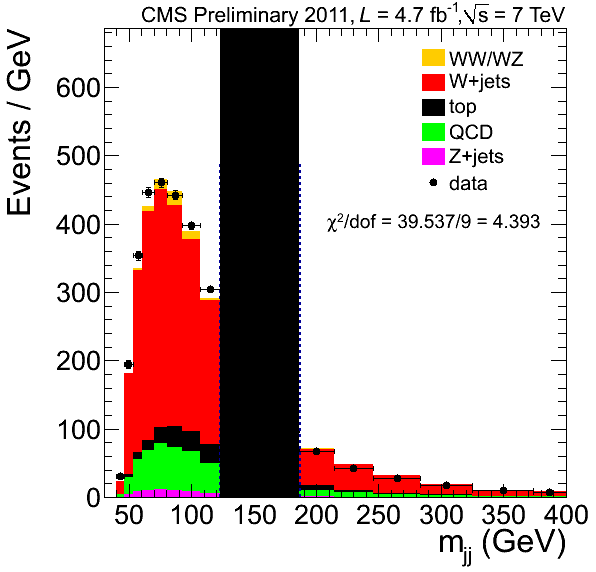
\includegraphics[width=0.45\textwidth]{figs/ElectronCuts/hist30_Wjj_Mjj_Electron_2jets_Stacked.png}
  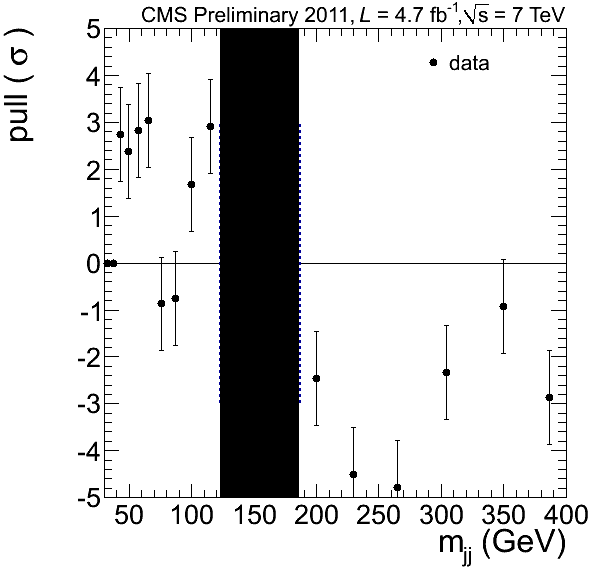
\includegraphics[width=0.45\textwidth]{figs/ElectronCuts/hist30_Wjj_Mjj_Electron_2jets_Pull.png}
\end{center}
\caption{\label{fig:Electron4030}Fit using MC shapes with lead jet cut at 40\,GeV and second jet cut at 30\,GeV.  The black bands are the points not included in the fit and are hidden so as not to bias the analysts' judgement.}
\end {figure}

To improve the agreement we increase the jet \pt thresholds and see
the effects.We use cuts of 40\,GeV and 40\,GeV, 45\,GeV and 45\,GeV,
and 50\,GeV and 50\,GeV.  This moves closer to the plateau of the
trigger turn on minimizing it sculpting of the distributions.  The
results of the fits are shown in
Figs.~\ref{fig:Electron4040}-\ref{fig:Electron5050}.  We select the
50\,GeV \pt cuts as the best.  The statistics of the data sample is
reduced from 44355 for the 40/30 cuts to 17017 for the 50/50 cuts.

\begin{figure}
\begin{center}
  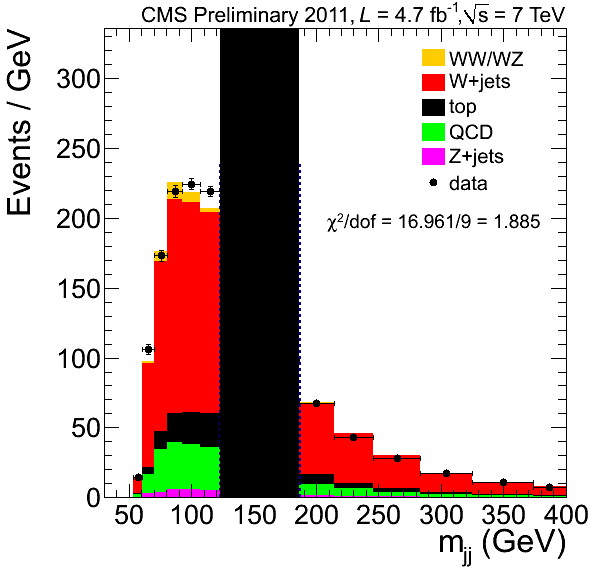
\includegraphics[width=0.45\textwidth]{figs/ElectronCuts/hist40_Wjj_Mjj_Electron_2jets_Stacked.png}
  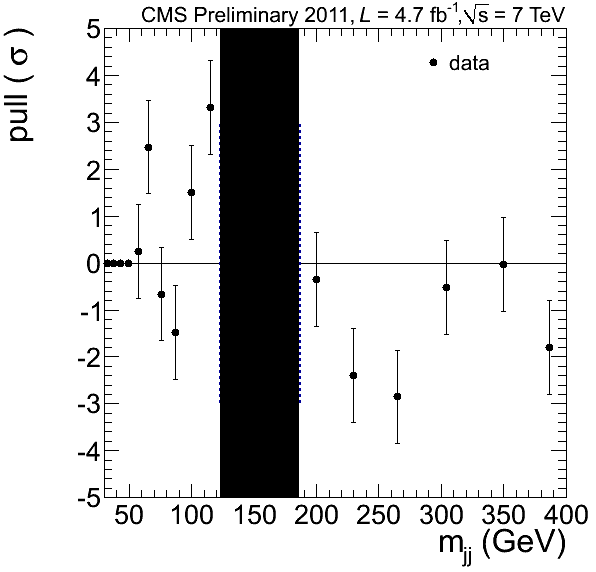
\includegraphics[width=0.45\textwidth]{figs/ElectronCuts/hist40_Wjj_Mjj_Electron_2jets_Pull.png}
\end{center}
\caption{\label{fig:Electron4040}Fit using MC shapes with lead jet cut
at 40\,GeV and second jet cut at 40\,GeV.  The black bands are the
points not included in the fit and are hidden so as not to bias the
analysts' judgement.}
\end {figure}

\begin{figure}
\begin{center}
  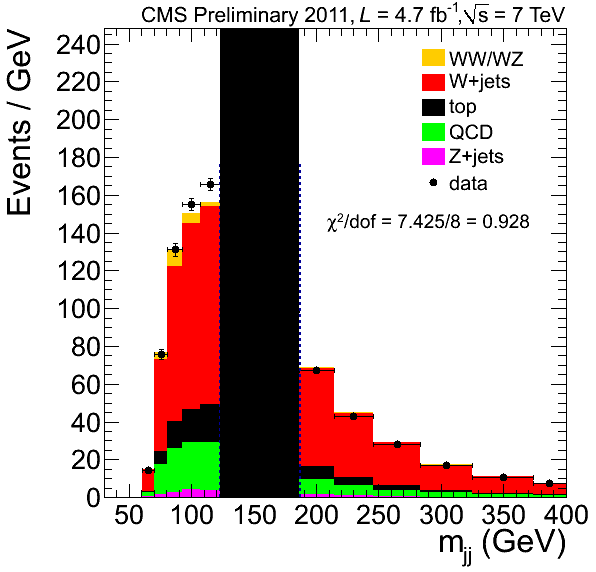
\includegraphics[width=0.45\textwidth]{figs/ElectronCuts/hist45_Wjj_Mjj_Electron_2jets_Stacked.png}
  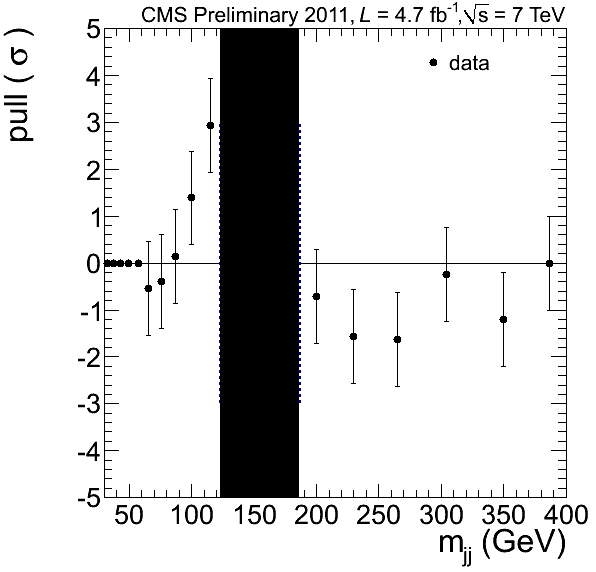
\includegraphics[width=0.45\textwidth]{figs/ElectronCuts/hist45_Wjj_Mjj_Electron_2jets_Pull.png}
\end{center}
\caption{\label{fig:Electron4545}Fit using MC shapes with lead jet cut at 45\,GeV and second jet cut at 45\,GeV.  The black bands are the points not included in the fit and are hidden so as not to bias the analysts' judgement.}
\end {figure}

\begin{figure}
\begin{center}
  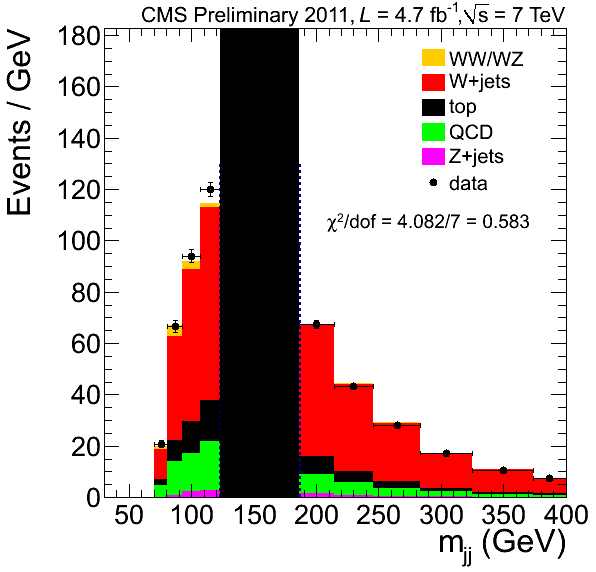
\includegraphics[width=0.45\textwidth]{figs/ElectronCuts/hist50_Wjj_Mjj_Electron_2jets_Stacked.png}
  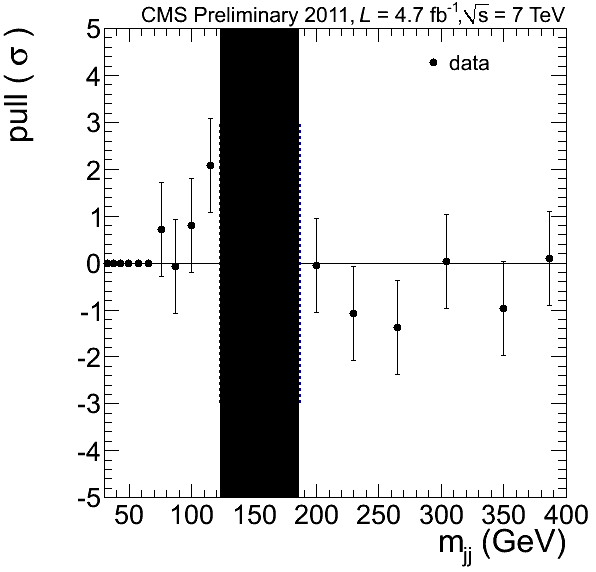
\includegraphics[width=0.45\textwidth]{figs/ElectronCuts/hist50_Wjj_Mjj_Electron_2jets_Pull.png}
\end{center}
\caption{\label{fig:Electron5050}Fit using MC shapes with lead jet cut at 50\,GeV and second jet cut at 50\,GeV.  The black bands are the points not included in the fit and are hidden so as not to bias the analysts' judgement.}
\end {figure}

These can be compared with the parameterized fit with the 40/30 cuts
shown in Fig.~\ref{fig:ElectronParam}.

\begin{figure}
\begin{center}
  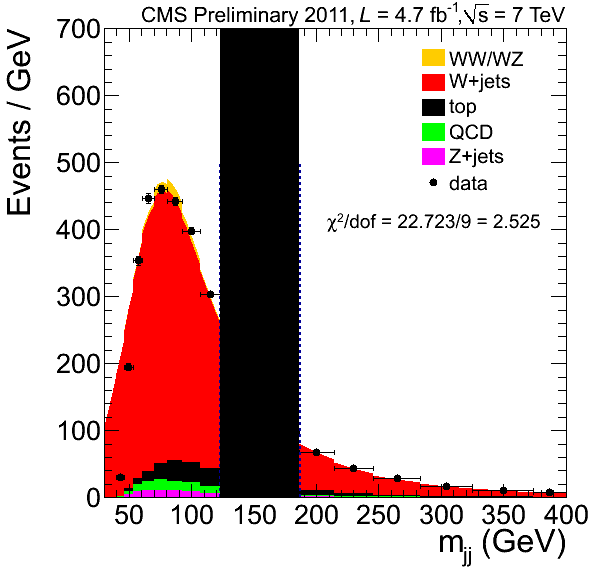
\includegraphics[width=0.45\textwidth]{figs/ElectronCuts/Params_Wjj_Mjj_Electron_2jets_Stacked.png}
  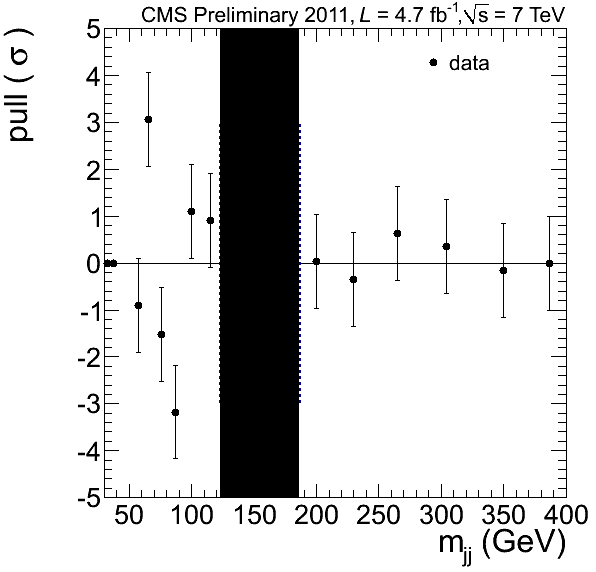
\includegraphics[width=0.45\textwidth]{figs/ElectronCuts/Params_Wjj_Mjj_Electron_2jets_Pull.png}
\end{center}
\caption{\label{fig:ElectronParam}Fit using MC shapes with lead jet cut at 40\,GeV and second jet cut at 30\,GeV.  The black bands are the points not included in the fit and are hidden so as not to bias the analysts' judgement.}
\end {figure}
